\documentclass[twocolumn,a4paper]{article}

\usepackage{geometry}
\usepackage{hyperref}
\usepackage{enumitem}
\usepackage{tikz}
\usepackage{pgfplots}
\usepackage{amsmath}
\usepackage{colortbl}
\usepackage{mathpazo}
\usepackage{microtype}

\title{Exploring the Efficiency of Covering Locality-Sensitive Hashing}

\author{
  Kasper Kronborg Isager \\
  IT University of Copenhagen, Denmark \\
  \texttt{kasi@itu.dk}
  \and
  Radoslaw Niemczyk \\
  IT University of Copenhagen, Denmark \\
  \texttt{radn@itu.dk}
}

\date{\today}

\geometry{
  margin = 12mm,
  footskip = 6mm,
  columnsep = 9mm
}

\usetikzlibrary{
  matrix,
  positioning
}

\setlist{noitemsep}

\pgfplotsset{compat=1.9}

\newtheorem{definition}{Definition}
\newtheorem{example}{Example}

\begin{document}
  \maketitle

  \begin{abstract}
One of the latest developments in the area of locality-sensitive hashing (LSH) is the so-called \textit{covering LSH} scheme. This scheme solves one of the primary drawbacks of classic locality-sensitive hashing, namely \textit{false negatives}, i.e. items that never collide with a query item despite them being similar. Covering LSH is therefore of interest in settings that require exact guarantees of producing a nearest neighbour, making classic LSH unsuitable as it only provides probabilistic guarantees. Given that the covering LSH scheme is still relatively new, it still lacks, to the best of our knowledge, a proper general-purpose implementation and associated evaluation thereof.

By implementing both the covering and the classic LSH schemes and benchmarking them on a real-world dataset designed for the evaluation of approximate nearest neighbour search algorithms, we show that within the same time and memory bounds, covering LSH is able to not only match but in fact outperform the filtering efficiency of classic LSH. This does however come at a negligible cost in insertion time and with an additional implementation specific memory overhead.
\end{abstract}

  \section{Introduction}
\label{introduction}

An increasingly popular approach for tackling similarity search in high-dimensional datasets is the so-called \textit{locality-sensitive hashing} (\textit{LSH}) technique, first presented by Piotr Indyk and Rajeev Motwani \cite{DBLP:conf/stoc/IndykM98}. LSH has therefore already found itself useful in a wide range of practical applications:

\begin{itemize}
  \item Nearest neighbour search
  \item Near-duplicate detection
  \item Hierarchical clustering
  \item Genome-wide association study
  \item Image and audio similarity identification
  \item Human fingerprint recognition
\end{itemize}

The basic idea of LSH is to hash items to \textit{buckets} in a way that provides a higher probability of similar items being hashed to the same bucket than dissimilar items. Items that then hash to the same bucket despite them being dissimilar are \textit{false positives}. On the other hand, similar items that never hash to the same bucket are \textit{false negatives} \cite[p. 88]{DBLP:books/cu/LeskovecRU14}. While false positives have no effect on the precision of queries, false negatives may cause the algorithm to never consider items that are in fact the most similar to a query item. The latter becomes a problem in settings that require exact rather than probabilistic guarantees of returning a nearest neighbour, as is the case in for example human fingerprint recognition.

A recent paper by Rasmus Pagh \cite{DBLP:journals/corr/Pagh15} proposes an LSH scheme that completely does away with false negatives at a cost in efficiency. The purpose of our paper is to compare this LSH scheme, named \textit{covering LSH}, with classic LSH on a number of different metrics such as query throughput and filtering efficiency.

\paragraph{Organisation} This paper is organised as follows: In section ~\ref{background} we provide the background for classic LSH and outline the covering LSH scheme and the guarantees that it provides. In section ~\ref{implementation} we describe our implementation of the two LSH schemes. In section ~\ref{evaluation} an experimental evaluation based on a real dataset is made after which we compare the two LSH schemes. Finally, in section ~\ref{conclusion} we give our parting thoughts on the covering LSH scheme and the cost of the exact guarantees that it provides.

  \section{Background}
\label{background}

As touched upon in section ~\ref{introduction}, locality-sensitive hashing tackles the problem of similarity search in high-dimensional datasets by relaxing the requirement of finding exact nearest neighbours. Instead, LSH is used as an \textit{approximate} nearest neighbour algorithm, which inherently implies only probabilistic guarantees of finding a nearest neighbour. In general, LSH act as a randomized filter that attempts to reduce an input set to a subset of candidates for a given query item.

The LSH schemes considered in this paper both operate in so-called \textit{Hamming space}:

\begin{definition}
\label{definition-hamming-space}
  A Hamming space $H(d, a)$ is the set of all words of length $d$ over an alphabet of size $a$. A distance measure over a Hamming space is the number of letters in which two words differ.
\end{definition}

The alphabet that we consider for LSH is $\{0, 1\}$ and words are therefore bit vectors of $d$ dimensions. The definition of the approximate nearest neighbour problem for Hamming space is given as follows in \cite{DBLP:journals/corr/PhamP16}:

\begin{definition}
\label{definition-nearest-neighbour}
  Given a set of vectors of dimensionality $d$ $Z \subset \{0, 1\}^d$, $|Z| = n$, the Hamming distance function $D$, a radius $r > 0$, an approximation factor $c > 1$, and a false negative rate $\delta > 0$, construct a data structure such that, given any query $q \in \{0,1\}^d$, if there exists $x \in Z$ and $D(x, q) \leq r$, it reports some $y \in Z$ where $D(y, q) \leq cr$ with probability $1 - \delta$.
\end{definition}

The data structure mentioned in definition ~\ref{definition-nearest-neighbour} makes use of a family of \textit{locality-sensitive hash functions} in order to hash items to buckets. The definition of this family is given as follows in \cite{DBLP:conf/stoc/IndykM98}:

\begin{definition}
\label{definition-hash-functions}
  Given $r > 0$, $c > 1$, and probabilities $p_1$ and $p_2$ where $p_1 < p_2$, a family $H$ is said to be $(r, cr, p_1, p_2)$-sensitive for $(Z, D)$ if for any $x, y \in Z$ we have

  \begin{itemize}
    \item if $D(x, y) \leq r$ then $Pr_H [h(x) = h(y)] \geq p_1$,
    \item if $D(x, y) > cr$ then $Pr_H [h(x) = h(y)] \leq p_2$.
  \end{itemize}
\end{definition}

Here, $p_1$ is the lower bound on the probability of close vectors colliding and $p_2$ is the upper bound on the probability of distant vectors colliding \cite[p. 100]{DBLP:books/cu/LeskovecRU14}. We therefore want $p_1$ to be close to 1 and $p_2$ to be close to 0.

\subsection{Classic LSH}
\label{background-classic-lsh}

The classic LSH family for Hamming space uses a random bit sampling approach for picking a number of components from an input vector. This sample is then used as the key in a map structure, which will be referred to as a \textit{partition}, for locating a bucket that the vector should be stored in. The bits to sample for a given partition are chosen independently and uniformly at random and stored with the partition. When looking for the nearest neighbour of a query vector, this sampling is repeated and the candidate vectors are those found in the bucket that the sample maps to.

\begin{example}
\label{example-classic-sampling}
  Given input vector $v = 1101$, we randomly chose to sample component 1 and 3, giving us the key $v' = 10$. We then proceed to update our map structure with an entry for this key: $10 \rightarrow \{1101\}$

  Given another input vector $u = 0110$, we again sample component 1 and 3, giving us the key $u' = 01$. We then add another entry to our map: $10 \rightarrow \{1101\}, 01 \rightarrow \{0110\}$.

  Given a query vector $q = 1001$, we once again sample component 1 and 3, giving us the key $q' = 10$. We then look up this key in our map and receive the following set of candidates: $\{1101\}$.
\end{example}

\begin{figure}[ht]
  \centering
  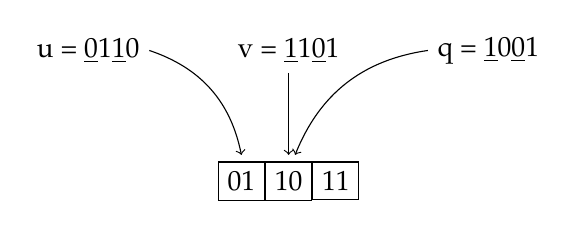
\begin{tikzpicture}
    \node (u) {u = \underline{0}1\underline{1}0};
    \node (v) [right=of u] {v = \underline{1}1\underline{0}1};
    \node (q) [right=of v] {q = \underline{1}0\underline{0}1};

    \matrix (m) [matrix of nodes, below=of v, row sep=-\pgflinewidth, style={nodes={draw}}]{
    01 & 10 & 11 \\
    };

    \path [->] (u.east) edge [bend left=30] ([yshift=0.5ex] m-1-1.north);
    \path [->] (v.south) edge ([yshift=0.5ex] m-1-2.north);
    \path [->] (q.west) edge [bend right=30] ([yshift=0.5ex, xshift=0.5ex] m-1-2.north);
  \end{tikzpicture}

  \caption{A graphical depiction of example ~\ref{example-classic-sampling}}
  \label{figure-classic-sampling}
\end{figure}

As can be seen in example ~\ref{example-classic-sampling}, $v$ and $u$ are not particularly similar as they only share a single component; by the sampling 1 and 3 they therefore do not map to the same bucket. However, $v$ and $q$ are almost identical as they share all but one component; the sampling 1 and 3 therefore maps them to the same bucket, albeit by chance. We have effectively reduced the set of potential candidates to half of the items in the original input set.

By adjusting the number of components sampled from vectors we can change the probability of collisions happening in the data structure. That is, by increasing the sample size we decrease the chance of vectors colliding, and vice versa, as more components would then have to match in order for a collision to happen.

If we want to keep the same sample size, but still increase the chance of vectors colliding, then we need to use more than one partition. Every partition will then independently chose the bits to sample and the set of candidate vectors will be the union of the vectors found in buckets in each partition.

\paragraph{Collision probabilities} By tweaking the sample size and the number of partitions to use, we can control the two probabilities $p_1$ and $p_2$ described in definition ~\ref{definition-hash-functions} \cite[p. 101]{DBLP:books/cu/LeskovecRU14}. By choosing a sample size $k$, the resulting probabilities will be $p_1^k$ and  $p_2^k$. On the other hand, by choosing a number of partitions 􏰄$l$, the resulting probabilities will be $1 - (1 - p_1)^l$ and $1 - (1 - p_2)^l􏰅$. By combining these, we get the probabilities $1 - (1 - p_1^k)^l$ and $1 - (1 - p_2^k)^l$, giving rise to what \cite[p. 89]{DBLP:books/cu/LeskovecRU14} calls the \textit{$S$-curve}:

\begin{figure}[ht]
  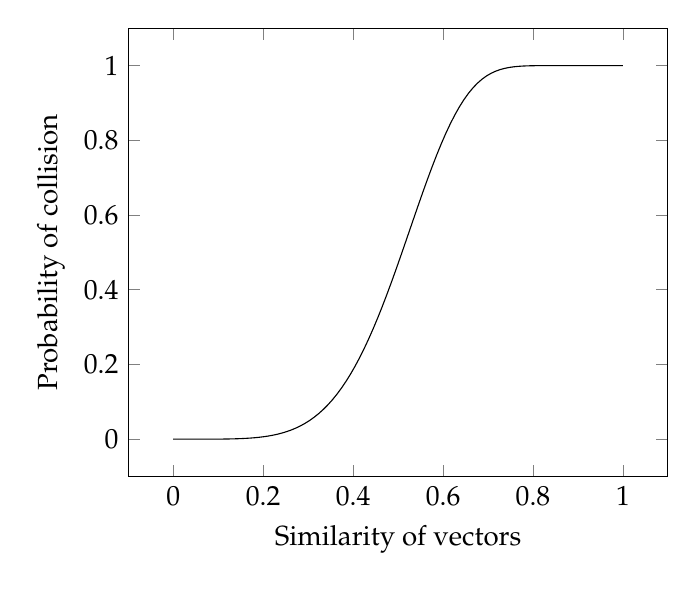
\begin{tikzpicture}
    \begin{axis}[
      xlabel = {Similarity of vectors},
      ylabel = {Probability of collision}
    ]
      \addplot[samples = 100, domain = 0:1]{1 - (1 - x^5)^20};
    \end{axis}
  \end{tikzpicture}

  \caption{The $S$-curve for $k = 5$, $l = 20$}
\end{figure}

\subsection{Covering LSH}
\label{background-covering-lsh}

Unlike the independently random bit sampling approach of classic LSH, covering LSH relies on a smarter sampling of correlated bits such that it can cover a given radius $r$. The difference between classic and covering LSH therefore lies in the family of hash functions used. The definition of a covering LSH family for Hamming space is given as follows in \cite{DBLP:journals/corr/PhamP16}:

\begin{definition}
\label{definition-covering-family}
  An LSH family $H$ is $r$-covering if for every two binary vectors $x, y \in \{0, 1\}^d$ with $D(x, y) \leq r$, there exists $h \in H$ such that $h(x) = h(y)$.
\end{definition}

A covering LSH family makes use of a random mapping $m \colon [d] \rightarrow \{0, 1\}^{r + 1}$ which constructs $d$ vectors, each consisting of $r + 1$ bits. This mapping is then used for constructing $2^{r + 1} - 1$ hash functions, or samplings, each associated with a different partition. In addition, each hash function is associated with a vector representation of $v \in \{1, \ldots, 2^{r + 1} - 1\}$. The bits to sample for each function in the family is determined by computing for each bit $b \in \{1, \ldots, d\}$, $m(b) \cdot v \bmod 2$, i.e. the dot product modulo 2 of $m(b)$ and $v$. If the result is 1, then the $b$th bit should be sampled.

\begin{example}
\label{example-covering-family}
  A 2-covering LSH family for $d = 4$ uses a random mapping $m \colon [4] \rightarrow \{0, 1\}^3$, e.g. $m(1) = 011, m(2) = 100, m(3) = 101, m(4) = 001$. This mapping is then used for constructing 7 hash functions, the first of which is $h(1)$:

  \begin{itemize}
    \item[] $b(1) = m(1) \cdot v \bmod 2 = 011 \cdot 001 \bmod 2 = 1$
    \item[] $b(2) = m(2) \cdot v \bmod 2 = 100 \cdot 001 \bmod 2 = 0$
    \item[] $b(3) = m(3) \cdot v \bmod 2 = 101 \cdot 001 \bmod 2 = 1$
    \item[] $b(4) = m(4) \cdot v \bmod 2 = 001 \cdot 001 \bmod 2 = 1$
  \end{itemize}

  $h(1)$ therefore samples bit 1, 3, and 4. This computation is repeated for the remaining hash functions, producing the following samplings:

  \begin{itemize}
    \item $h(2)$ samples bit 1
    \item $h(3)$ samples bit 3 and 4
    \item $h(4)$ samples bit 2 and 3
    \item $h(5)$ samples bit 1, 2, and 4
    \item $h(6)$ samples bit 1, 2, and 3
    \item $h(7)$ samples bit 2 and 4
  \end{itemize}
\end{example}

\begin{table}[h]
  \centering
  \begin{tabular}{c | c | c | c}
    & 1 & 2 & 3 \\
    \hline
    2 & $h(5)$, $h(6)$ & \cellcolor{gray!10} & \cellcolor{gray!10} \\
    \hline
    3 & $h(1)$, $h(6)$ & $h(4)$, $h(6)$ & \cellcolor{gray!10} \\
    \hline
    4 & $h(1)$, $h(5)$ & $h(5)$, $h(7)$ & $h(1)$, $h(3)$ \\
  \end{tabular}

  \caption{Depiction of how all possible combinations of 2 bits are covered by functions from the 2-covering family}
  \label{table-covering-family}
\end{table}

As can be seen from example ~\ref{example-covering-family}, which has been adapted from \cite[example 2.1]{DBLP:journals/corr/PhamP16}, and table ~\ref{table-covering-family}, a 2-covering LSH family for 4-dimensional vectors is able to "cover" all combinations of bit pairs. This in effect guarantees that no false negatives will be produced within the given radius of 2.

\paragraph{Constraints} The covering LSH family works under the assumption that $cr = \log n$. This constraint has in \cite{DBLP:journals/corr/Pagh15} been generalized to arbitrary values of $c$, $r$, and $n$ but we will not further touch upon these generalizations in this paper.

  \section{Implementation}
\label{implementation}

A library implementing both the classic and covering LSH schemes, as described in section ~\ref{background}, has been developed in order to facilitate an experimental evaluation of the two schemes. The library has been released as open-source software and is available at \url{https://github.com/kasperisager/hemingway}. C++ was chosen as the implementation language as it balances performance with higher-level constructs that help ensure a safe and succinct implementation. The library is fairly simple in that it only exposes two classes: One for representing bit vectors and one for representing the actual LSH data structure.

\subsection{Vector}

The vector class provides an efficient bit vector representation that allows for arbitrarily large dimensionality by storing bit components in a variable number of 32-bit integer chunks. This representation effectively supports all the operations needed by the LSH schemes:

\begin{itemize}
  \item Random access in $\mathcal{O}(1)$
  \item Distance computing in $\mathcal{O}(c)$
  \item Dot product computing in $\mathcal{O}(c)$
  \item Equality checking in $\mathcal{O}(c)$
  \item Hash computing in $\mathcal{O}(c)$
  \item Bitwise AND in $\mathcal{O}(c)$
\end{itemize}

Here, $c$ denotes the number of component chunks in a vector. The time complexity of each operation has been listed in order to justify the comparison between the two LSH schemes; as can be seen, no vector operation poses a bottleneck for neither scheme.

\paragraph{Equality and hash} The equality and hash operations are used for interoperation with the hash-based data structures of the C++ standard library. As such, they are not related to the concept of hashing in LSH.

\paragraph{Bitwise AND} The bitwise AND operation is used for performing the bit sampling described in section ~\ref{background}. For example, to sample bit 1 and 3 of a vector $v = 1101$, we construct a separate vector \textit{mask} $u = 1010$, i.e. a vector with bit 1 and 3 set. The key is then be the bitwise AND of $v$ and $u$, $1101 \wedge 1010 = 1000$. As can be seen, this is analogous to the key $v' = 10$ from example ~\ref{example-classic-sampling} when bit 2 and 4 are removed.

\paragraph{Population counts} It is assumed in \cite{DBLP:journals/corr/Pagh15} that population counts, i.e. the number of 1s in a set of bits, can be counted in $\mathcal{O}(1)$. The \texttt{\_\_builtin\_popcount}\footnote{\url{https://gcc.gnu.org/onlinedocs/gcc/Other-Builtins.html}} intrinsic supports this and is used in the library, hence complexity $\mathcal{O}(c)$ of the distance, equality, dot product, and bitwise AND operations.

\subsection{Table}

The table class provides a representation of the LSH data structure itself and is constructed by supplying a configuration for either the classic or covering LSH scheme. In the case of classic LSH, the number of bits to sample from vectors and the number of partitions to use are specified. In the case of covering LSH, the radius is specified.

When configuring the table, the notion of the parameters $r$, $c$, and $\delta$ from definition ~\ref{definition-nearest-neighbour} is by design left out. The onus of picking parameters appropriate for a given input set and use case is therefore on the client of the library. As a consequence, the data structure also doesn't require specifying the size $n$ of the input set at construction time.

\paragraph{Operations} Once configured, vectors can be inserted into and erased from the table using an API similar to that of most data structures in the C++ standard library. Query operations can then be performed against the table once filled with data. A query operation will always return the closest vector found, regardless of the approximation factor $c$ from ~\ref{definition-nearest-neighbour}. This is again by design, leaving open the option of the client interpreting the result however they see fit.

\paragraph{Internals} Internally, the table consists of several partitions, each represented as a mapping from vector keys to buckets. When adding a vector to the table, this vector is assigned a unique integer identifier and stored in the table. The identifier of the vector is then stored in an associated bucket in each of the different partitions in order to avoid copying the vector itself to every partition. The key used for associating a vector with a bucket is constructed differently depending on the configured LSH scheme, but this is in essence the only functional difference between the two schemes.

\paragraph{Hashing} Both LSH schemes make use of the Mersenne Twister pseudorandom number generator when constructing hash functions, ensuring a uniform distribution as required by \cite{DBLP:conf/stoc/IndykM98} and \cite{DBLP:journals/corr/Pagh15}. The random number generator is in classic LSH used for setting $k$ random bits in vector masks, whereas it is in covering LSH used for setting random bits in vectors for the mapping $m$.

  \section{Evaluation}
\label{evaluation}

The following section will provide an evaluation of the two schemes based on an automated benchmark implemented as part of the C++ library described in section ~\ref{implementation}. The benchmark measures the following metrics of each LSH scheme:

\begin{itemize}
  \item \textbf{Insertion throughput:} How many items can be inserted into the data structure per second on average?
  \item \textbf{Query throughput:} How many queries can be performed against the data structure per second on average?
  \item \textbf{Bucket distribution:} How many buckets are created per partition on average?
  \item \textbf{False negative rate:} How many false negatives occur per query on average?
\end{itemize}

The benchmark performs a 1-NN search in each of three configured tables: A brute force table, a classic table, and a covering table. The purpose of the brute force table is to establish the ground truth by locating the exact nearest neighbour for each of the query items. This ground truth is then used for determining if a false negative has been encountered for each of the query results in the classic and covering tables.

\textbf{Note:} The construction time of the data structure itself under the different schemes is not considered by the benchmark, as we consider this a pre-processing step. However, the construction time required for covering LSH is significantly higher than that required by classic LSH due to the increased complexity of constructing covering families of hash functions. This issue is tackled in \cite{DBLP:journals/corr/PhamP16} which proposes the so-called \textit{fast covering LSH} scheme for efficiently constructing covering families.

\paragraph{Dataset} The dataset used for the evaluation is a pre-processed version of the \texttt{ANN\_SIFT1M} set distributed as part of the Multi Index Hashing (MIH) library located at \url{https://github.com/norouzi/mih}.

This dataset is created specifically for the evaluation of approximate nearest neighbour search algorithms and is a set of 1 million image feature vectors of 128 dimensions, plus an additional 10,000 query vectors. The version distributed alongside the MIH library is however binarised to vectors of 64 dimensions using LSH, which better suits the purpose of our evaluation.

\paragraph{Parameters} Our choice of parameters follows that of the experiments carried out in \cite{DBLP:journals/corr/PhamP16}. That is, for a given radius $r$, we set the number of partitions to use in the classic table to $l = 2^{r + 1} - 1$ and the number of bits to sample to $k = 􏰢\frac{\log(1 - \delta^{\frac{1}{l}})}{\log(1 - \frac{r}{d})}$.􏰣 The benchmark is run for both $\delta = 0.01$ and $\delta = 0.001$. For the covering table we just need the radius $r$.

\subsection{Results}

The results were obtained by running the benchmark on a 2.8 GHz Intel Core i5 processor with a 3 MB L3 cache and 8 GB of DDR3 memory. Due to the limited amount of memory available, we have only been able to provide results for $r \in \{2,\ldots,5\}$.

\subsubsection{Bucket distribution}

We start by considering the average number of buckets created per partition as this turned out to be the defining difference between the two LSH schemes. As can be seen in figure ~\ref{fig:buckets-per-partition}, the average number of buckets per partition is in the case of classic LSH dependent on the radius, and as such the number of bits sampled.

This, however, is not the case in covering LSH where the number of buckets per partition remains constant for every radius. This ties into the way covering LSH correlates the bits to sample from vectors, causing the number of buckets per partition to depend on the input set rather than the radius.

The increased number of buckets does however cause an increase in the total memory usage of the data structure, as each bucket in our implementation has an overhead of 24 bytes on a 64-bit operating system.

\begin{figure}[ht]
  \centering
  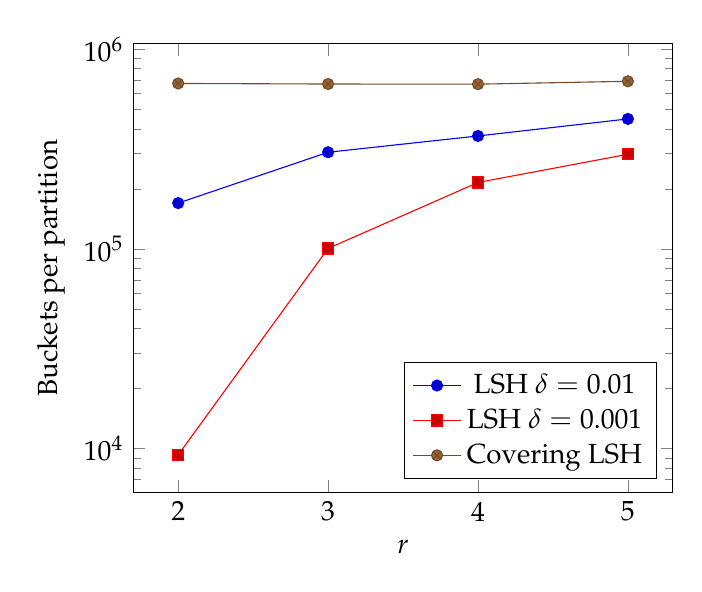
\begin{tikzpicture}
    \begin{semilogyaxis}[
      xlabel = {$r$},
      ylabel = {Buckets per partition},
      xtick = data,
      legend pos = south east
    ]
      \addplot coordinates {
        (2, 169815.43)
        (3, 305179.47)
        (4, 368261.81)
        (5, 448140.33)
      };

      \addplot coordinates {
        (2, 9310.57)
        (3, 100652.33)
        (4, 215357.87)
        (5, 298153.22)
      };

      \addplot coordinates {
        (2, 674554.00)
        (3, 670221.60)
        (4, 669083.68)
        (5, 691636.11)
      };

      \legend{LSH $\delta = 0.01$, LSH $\delta = 0.001$, Covering LSH}
    \end{semilogyaxis}
  \end{tikzpicture}

  \caption{Comparison of bucket distribution}
  \label{fig:buckets-per-partition}
\end{figure}

\subsubsection{Insertion throughput}

As can be seen in figure ~\ref{fig:insertions-per-second}, the insertion throughput of the two LSH schemes follows the same trend as the bucket distribution, albeit in reverse. As such, covering LSH performs worse than classic LSH due to the added overhead of having to construct more buckets. While the difference in bucket distribution is rather significant between the two schemes, the difference in insertion time is negligible in comparison.

\begin{figure}[ht]
  \centering
  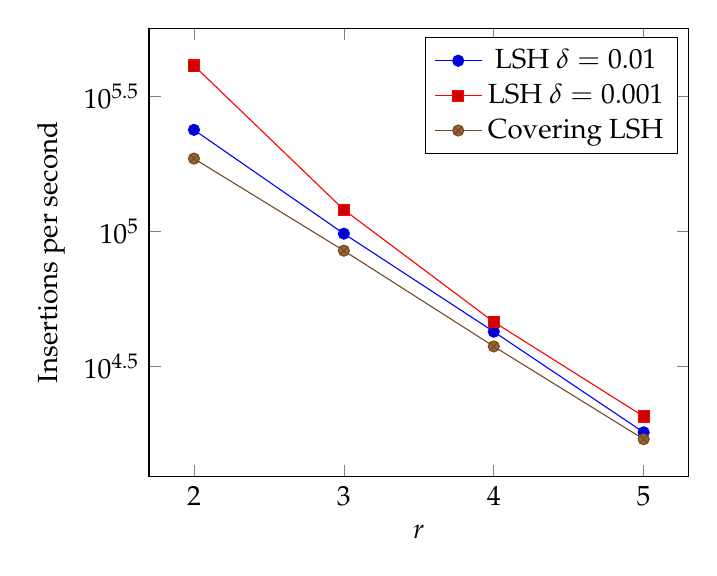
\begin{tikzpicture}
    \begin{semilogyaxis}[
      xlabel = {$r$},
      ylabel = {Insertions per second},
      xtick = data
    ]
      \addplot coordinates {
        (2, 237736.94)
        (3, 98187.51)
        (4, 42593.97)
        (5, 18074.10)
      };

      \addplot coordinates {
        (2, 411106.15)
        (3, 120359.67)
        (4, 46280.57)
        (5, 20693.81)
      };

      \addplot coordinates {
        (2, 186131.05)
        (3, 84934.71)
        (4, 37573.59)
        (5, 17047.07)
      };

      \legend{LSH $\delta = 0.01$, LSH $\delta = 0.001$, Covering LSH}
    \end{semilogyaxis}
  \end{tikzpicture}

  \caption{Comparison of insertion throughput}
  \label{fig:insertions-per-second}
\end{figure}

\subsubsection{Query throughput}

Our initial expectations of the query throughput of the covering LSH scheme was that it would follow the same trend as the insertion throughput, i.e. be slightly less performant than the query throughput of classic LSH. As seen in figure ~\ref{fig:queries-per-second}, this is however far from the case. Due to the bucket distribution of covering LSH, we can assume that it is able to produce candidate sets that on average are smaller than those produced by classic LSH. The improved filtering efficiency in turn has a significant effect on the query throughput, making covering LSH perform much better than classic LSH on the evaluated dataset.

\begin{figure}[ht]
  \centering
  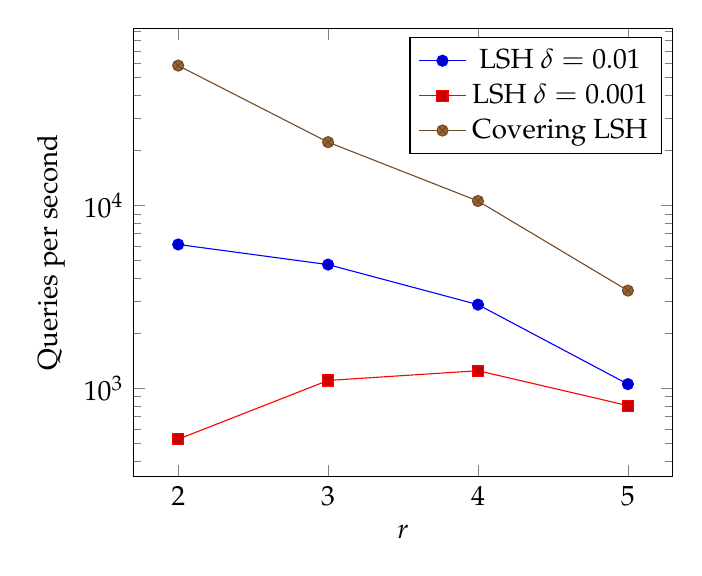
\begin{tikzpicture}
    \begin{semilogyaxis}[
      xlabel = {$r$},
      ylabel = {Queries per second},
      xtick = data
    ]
      \addplot coordinates {
        (2, 6118.88)
        (3, 4747.76)
        (4, 2866.80)
        (5, 1053.48)
      };

      \addplot coordinates {
        (2, 526.67)
        (3, 1103.17)
        (4, 1247.75)
        (5, 803.80)
      };

      \addplot coordinates {
        (2, 58216.55)
        (3, 22187.94)
        (4, 10574.71)
        (5, 3421.63)
      };

      \legend{LSH $\delta = 0.01$, LSH $\delta = 0.001$, Covering LSH}
    \end{semilogyaxis}
  \end{tikzpicture}

  \caption{Comparison of query throughput}
  \label{fig:queries-per-second}
\end{figure}

\subsubsection{False negative rates}

The last metric considered is the false negative rates of the two LSH schemes. As can be seen in figure ~\ref{fig:false-negatives-per-query}, the number of false negatives per query is exactly as one would expect; classic LSH produces false negatives proportional to $\delta$ and covering LSH produces no false negatives at all, as is also shown by the experiments conducted in \cite{DBLP:journals/corr/PhamP16}.

While classic LSH with $\delta = 0.001$ does provide low probabilities of false negatives, it does so at a major decrease in query throughput as witnessed by figure ~\ref{fig:queries-per-second}. The query throughput of classic LSH with delta $\delta = 0.01$ comes closer to that of covering LSH, but this of course at an increased rate of false negatives.

\begin{figure}[ht]
  \centering
  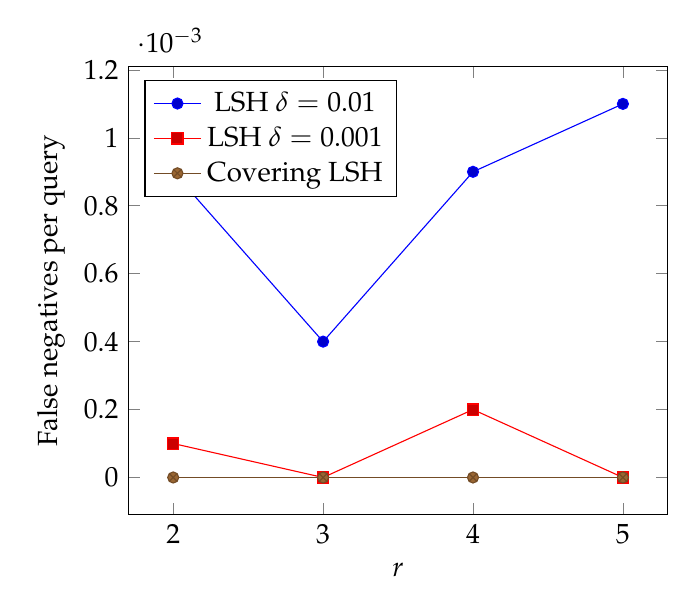
\begin{tikzpicture}
    \begin{axis}[
      xlabel = {$r$},
      ylabel = {False negatives per query},
      xtick = data,
      legend pos = north west
    ]
      \addplot coordinates {
        (2, 0.0009)
        (3, 0.0004)
        (4, 0.0009)
        (5, 0.0011)
      };

      \addplot coordinates {
        (2, 0.0001)
        (3, 0.0000)
        (4, 0.0002)
        (5, 0.0000)
      };

      \addplot coordinates {
        (2, 0.0000)
        (3, 0.0000)
        (4, 0.0000)
        (5, 0.0000)
      };

      \legend{LSH $\delta = 0.01$, LSH $\delta = 0.001$, Covering LSH}
    \end{axis}
  \end{tikzpicture}

  \caption{Comparison of false negative rates}
  \label{fig:false-negatives-per-query}
\end{figure}

  \section{Conclusion}
\label{conclusion}

We have in this paper shown how the proposed covering LSH scheme performs compared to the classic LSH scheme when both are implemented as part of a general-purpose C++ library. Based on our evaluation, we can conclude that the query throughput of covering LSH outperforms that of classic LSH given the same time and memory bounds. This as a result of an improved distribution of items in buckets across partitions, which in turn reduces the average size of candidate sets for query items. The improved filtering efficiency does however come at a cost in the form of a decrease in insertion time and an additional memory overhead, both caused by the increased number of buckets.

In addition, our results verify the claim made in \cite{DBLP:journals/corr/Pagh15} that the efficiency of the covering LSH scheme matches that of the classic LSH scheme of \cite{DBLP:conf/stoc/IndykM98} in the case that $cr = \log n$. As stated earlier, the efficiency of our implementation in fact surpasses that of the classic LSH scheme while maintaining the exact guarantees of producing a nearest neighbour.


  \bibliographystyle{abbrv}
  \bibliography{tex/bibliography}
\end{document}
